\documentclass[12pt]{article}

\usepackage{mathpazo}

\usepackage{amsmath}
\usepackage{amssymb}
\usepackage{xcolor}
\usepackage{graphicx}
\usepackage[alsoload=binary]{siunitx}
\usepackage{booktabs}
\usepackage{multirow}
\usepackage{fancyvrb}
\usepackage[section]{placeins}
\usepackage{flafter}
\usepackage{url}
\usepackage{hyperref}

% make plots
\usepackage{pgfplots}

% a bit more compact
\renewcommand\l{\mathopen{}\left}
\renewcommand\r{\right}

% no section numbers
\setcounter{secnumdepth}{-2}

% leave notes to yourself
\newcommand\todo[1]{\textcolor{red}{\textsc{todo}: #1}}

\newcommand\abs[1]{\l\vert #1 \r\vert}
\newcommand\grad[1]{\nabla #1}
\newcommand\lap[1]{\nabla^2 #1}
\let\epsilon\varepsilon

\usepackage{bm}
\renewcommand\vec[1]{\bm{#1}}
\newcommand\unit[1]{\hat{\vec{#1}}}

\bibliographystyle{elsarticle-num}

\title{Phase Field Modeling of Solidification}
\author{Sam Britt}
\date{December 14, 2012}

\begin{document}
\maketitle

\section{Introduction}
Solidification is an important step in materials processing---both
during the initial processing and during fabrication steps such as
welding---and remains an active area of research. A variety of
complex processes can and do occur during solidification, such as the
nucleation, growth, and impingement of precipitates, the segregation
of solute in the solid and the melt, and the formation of complex
morphologies such as eutectic segregation, columnar grains, and
dendritic growth. The occurrence of such processes has implications on
the subsequent processing steps (e.g., an annealing step may be
necessary due to solute segregation), and, depending on the morphology
of the material after solidification, subsequent mechanical working
may become more difficult or costly.

Thus, understanding and, to the extent possible, predicting the
solidification characteristics of an alloy system is great interest to
materials engineers. Consider a solid precipitate growing in the
liquid matrix. There are three entities to consider: the solid, the
liquid, and the interface between them. To describe the solidification
front is to solve, at each interface, equations involving heat and
solute diffusion in the solid, heat and solute diffusion in the
liquid, energy conservation at the interface, total conservation of
solute via transport equations across the interface, and the
Gibbs-Thomson capillarity equation at the interface to account for the
effect of interface curvature~\cite{Qin2010}. This assumes no
convection in the liquid, and of course the location each interface
must be tracked explicitly through the simulation. The computational
demands of this so-called ``sharp interface'' model limits its
applicability.

In contrast, the phase field model forgoes many of the above
considerations and uses just a few equations, sacrificing some rigor
for efficiency and broader applicability. The key to the approach
is the ``order parameter" $\phi$, a field variable which takes values
between $0$ and $1$. Instead of explicitly modeling solid, liquid and
interface, $\phi$ takes on the value $0$ where the system is in the
solid state and $1$ where the system is liquid (or vice versa,
depending on convention). Where $\phi$ changes continuously from $0$
to $1$ is said to be the ``interface''. This results in a diffuse
interface between solid and liquid, see
Figure~\ref{fig:diffuse-interface}. Now, the interface no longer needs
to be tracked explicitly, but rather $\phi$ is allowed to evolve in
time. The location of the interface in the simulation space is simply
a byproduct.

\begin{figure}[htbp]
  \centering
  \begin{minipage}[t]{.8\linewidth}
    \centering
    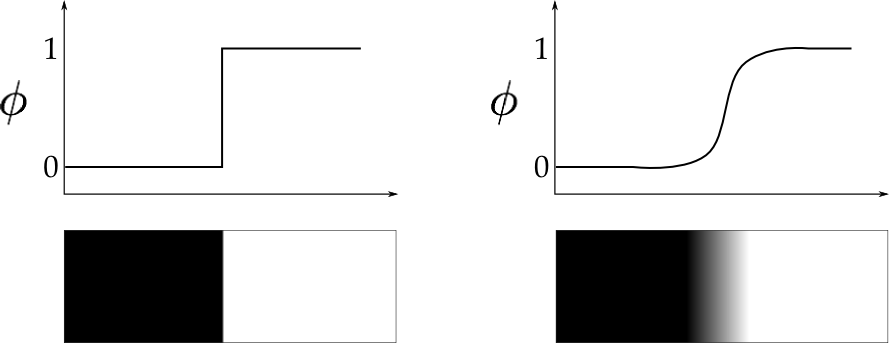
\includegraphics[width=\linewidth]{img/diffuse_interface}
    \caption{Contrast between the sharp interface model (left) and the
    phase field model. In the sharp interface model, there is a
    discontinuity of phase between solid (dark) and liquid (white). In
    the phase field model, the continuous change in $\phi$ results in
    a diffuse interface between solid and liquid.}
    \label{fig:diffuse-interface}
  \end{minipage}
\end{figure}


\section{The Phase Field Model}
The treatment of the phase field model begins with the free energy
functional for a pure material \cite{Chen2002,Boettinger2002},
\begin{equation}
  \label{eq:free-energy}
  F = \int_V \l[
    f(\phi, T)
    +
    \frac{\epsilon^2}{2} \abs{\grad\phi}^2
  \r]
  dV.
\end{equation}
$F$ here is the Gibbs free energy of the bulk, $f(\phi, T)$ is the
local free energy density, and $\epsilon$ is called the interfacial
gradient free energy coefficient. Many other terms can be added to
Eqn.~\eqref{eq:free-energy} if they are believed to have significant
 effect on free energy; in particular, a composition-dependent term
should be added for multi-component systems. Note that the second term
on the right hand side of Eqn.~\eqref{eq:free-energy} is only non-zero
at the interface---it captures the effect of the interface on free
energy, where the first term is the contribution from the solid and
liquid phases individually.

To ensure that the free energy is reduced over time for this
(irreversible) process, the following form for evolution of $\phi$ is
used \cite{Qin2010}
\begin{equation}
  \label{eq:allen-cahn}
  \frac{\partial \phi}{\partial t}
  = M
  \l[
    \epsilon^2 \lap{\phi}
    -\frac{\partial f(\phi, T)}{\partial \phi}
  \r],
\end{equation}
where $M$ is called the interfacial mobility. This is often coupled
with the heat equation for non-isothermal treatments of solidification
\begin{equation}
  \label{eq:heat-eqn}
  \frac{\partial u}{\partial t}
  = D \lap u +
  \frac{1}{2} \frac{\partial \phi}{\partial t}
\end{equation}
where $u$ is a normalized temperature defined as
\begin{equation*}
  u \equiv \frac{T - T_m}{L / c_P}.
\end{equation*}
where $T_m$ is the equilibrium melting temperature, $L$ is the latent
heat of fusion, and $c_P$ is the heat capacity.

The local free energy density $f(\phi, T)$ is treated as an
interpolation between the free energy densities of the solid and
liquid phases, $f_S$ and $f_L$, respectively, along with an activation
energy $Q$ to capture the fact that the liquid is metastable in this
undercooled ($T < T_m$) state. The energy density is written as
\begin{align}
  f(\phi, T) &= \l[ 1 - p(\phi) \r] f_S(T) + p(\phi) f_L(T) + Q g(\phi) \notag
  \\
          &= f_S(T) + p(\phi) \l[f_L(T) - f_S(T)\r]+ Q g(\phi)
  \label{eq:bulk_energy}
\end{align}
The functions $p(\phi)$ and $g(\phi)$ are plotted in
Figure~\ref{fig:p_and_g};  $p(\phi)$ is an interpolation
function and $g(\phi)$ is a double-well function, written as
\begin{align}
     p(\phi) &= \phi^3 \l( 6 \phi^2 - 15\phi + 10 \r) \notag \\
     g(\phi) &= \phi^2 \l( 1 - \phi \r)^2. \notag
\end{align}


\begin{figure}[htbp]
  \centering
  \begin{minipage}[t]{.7\linewidth}
    \centering
    \begin{tikzpicture}
      \begin{axis}
        [
          domain=-0.1:1.1,
          ymin=0,
          ymax=1,
          no markers,
          xlabel=$\phi$,
          ylabel=$10 g(\phi)$ or $p(\phi)$,
          samples=100,
          legend style={
            at={(0.03,0.97)},
            anchor=north west
          }
        ]
        \addplot expression {10*x^2 * (1 - x)^2};             % 10 g(phi)
        \addplot expression {x^3 * (6* x^2 - 15 * x + 10)};   % p(phi)
        \legend{$10 g(\phi)$,$p(\phi)$}
      \end{axis}
    \end{tikzpicture}
    \caption{The functions $p(\phi)$ and $g(\phi)$. The values of $g$
    have been scaled for clarity.}
    \label{fig:p_and_g}
  \end{minipage}
\end{figure}

The expression for $f(\phi, T)$ can be simplified by in two ways:
\begin{enumerate}
  \item Since we only require \emph{changes} in free energy, set solid
    as standard state, so that, for all $T$
    \begin{equation*}
      f_S(T) \equiv 0.
    \end{equation*}
  \item Use the common approximation for alloys at $T \approx T_m$
    \cite{Porter1992}
    \begin{align*}
      \Delta f_{\text{melt}} = f_L(T) - f_S(T)
      &\approx \frac{L \l( T_m - T \r)}{T_m} \\
      &= - \frac{L^2}{c_P T_m} u \\
      &= - \kappa u
    \end{align*}
    where $\kappa = L^2/ \l( c_P T_m \r)$.
\end{enumerate}
Therefore, changing from $T$ to $u$ and substituting
into~\eqref{eq:bulk_energy}, we have
\begin{equation}
  \label{eq:bulk_energy_solved}
  f(\phi, u) = - \kappa u p(\phi) + Q g(\phi).
\end{equation}

In one dimension, the interface thickness $\delta$ is given by
\begin{equation}
  \label{eq:interface-thickness}
  \delta = \frac{\epsilon}{\sqrt{2 Q}}
\end{equation}
and the surface free energy $\sigma$ is
\begin{equation*}
  \sigma = \frac{\epsilon \sqrt{Q}}{3 \sqrt{2}}.
\end{equation*}

To introduce anisotropy, necessary for modeling, e.g., dendritic
structures, let $\epsilon = \epsilon(\unit{n})$, where $\unit{n}$ is
the unit vector normal to the to the interface.
Following \cite{Bragard2002},
\begin{equation*}
  \epsilon^2\l( \unit n \r)
    = \epsilon_0^2
        \l( 1 - 3 \epsilon_c \r)
        \l[
          1  + \frac{4 \epsilon_c}{1 - 3 \epsilon_c}
          \l(
            n_x^4 + n_y^4 + n_z^4
          \r)
        \r]
\end{equation*}
where $\epsilon_c$ is a constant, $\epsilon$ reduces to $\epsilon_0$
in the isotropic case, and $\unit n$ is
taken as $- \grad \phi / \abs{ \grad \phi }$, so that
\begin{equation*}
  n_x^4 + n_y^4 + n_z^4 =
  \frac{
    \l( \partial \phi / \partial x \r)^4 +
    \l( \partial \phi / \partial y \r)^4 +
    \l( \partial \phi / \partial z \r)^4
  }{
    \abs{ \grad \phi }^4
  }.
\end{equation*}

\section{Numerical Analysis}
Finding the derivative of Eqn.~\eqref{eq:bulk_energy_solved} and
substituting into~\eqref{eq:allen-cahn}, we have
\begin{equation*}
  \frac {\partial \phi }{ \partial t } =
  M \epsilon^2 \lap{\phi} +
  2 M \phi \l[ 
    15 \kappa u \phi \l( \phi - 1 \r)^2 -
    Q \l( 1 - \phi \r) \l( 1 - 2 \phi \r)
  \r]
\end{equation*}
Let $h\l( \phi, u \r)$ be the second term on the right hand side of
the above equation, so
\begin{equation}
  \frac {\partial \phi }{ \partial t }
  = M \epsilon^2 \lap{\phi} + h\l( \phi, u \r),
  \label{eq:dphidt}
\end{equation}
which is to be integrated numerically, coupled with
Eqn.~\eqref{eq:heat-eqn} for non-isothermal simulations.

For this work, Eqn.~\eqref{eq:dphidt} was solved in the isothermal
case for a pure system in one dimension. Attempts to extend the
solution were met with difficulties in convergence which is believed
to be due to the values of the coefficients ($\epsilon$, $M$, $Q$)
coupled with the physical parameters $T_m$, $c_P$, and $L$. Attempts
to base these coefficients in terms of real physical quantities
perhaps introduces instabilities into the solution.

Equation~\eqref{eq:dphidt} was expanded and rewritten in terms of
finite differences. A central finite difference was used for the $\lap
\phi$ term. A forward difference for $\partial \phi / \partial t$ was
first attempted (explicit scheme) but the resulting timesteps needed
for convergence were vanishingly small. A fine spacial discretization
is required for phase field modeling, because the interface---where
$\phi$ changes quite rapidly---is the primary feature of interest.
After re-writing $\partial \phi / \partial t$ with backward finite
difference (implicit scheme), Eqn.~\eqref{eq:dphidt} becomes a
tridiagonal system of equations that must be solved at each timestep.
This system was solved in different ways through the course of the
project: using a LAPACK subroutine, using a Cholesky decomposition
algorithm built in-house, and parallelizing the solution of the
system, where each node computes on a column of the matrix and passes
its results to the next node. Speedup was not detected using such a
scheme.

Figures~\ref{fig:esp1M.5},~\ref{fig:esp1M1}, and~\ref{fig:esp2M.5}
show the evolution of $\phi$ with time for different choices of
$\epsilon$ and $M$. Here, $\phi=1$ implies the solid phase. Comparing
Figures~\ref{fig:esp1M.5} and~\ref{fig:esp1M1}, we see the effect that
$M$ has on the speed of the solidification process. Comparing
Figures~\ref{fig:esp1M.5} and~\ref{fig:esp2M.5}, we see that the
energy gradient coefficient $\epsilon$ has not only affect the speed
of the solidification process, but also the interface thickness,
consistent with Eqn.~\eqref{eq:interface-thickness}. It is these types
of parameter studies, especially when the parameters can be related to
physical quantities, that can give materials engineers insight into
the solidification process.

\begin{figure}[htbp]
  \centering
  \begin{minipage}[t]{.8\linewidth}
    \centering
    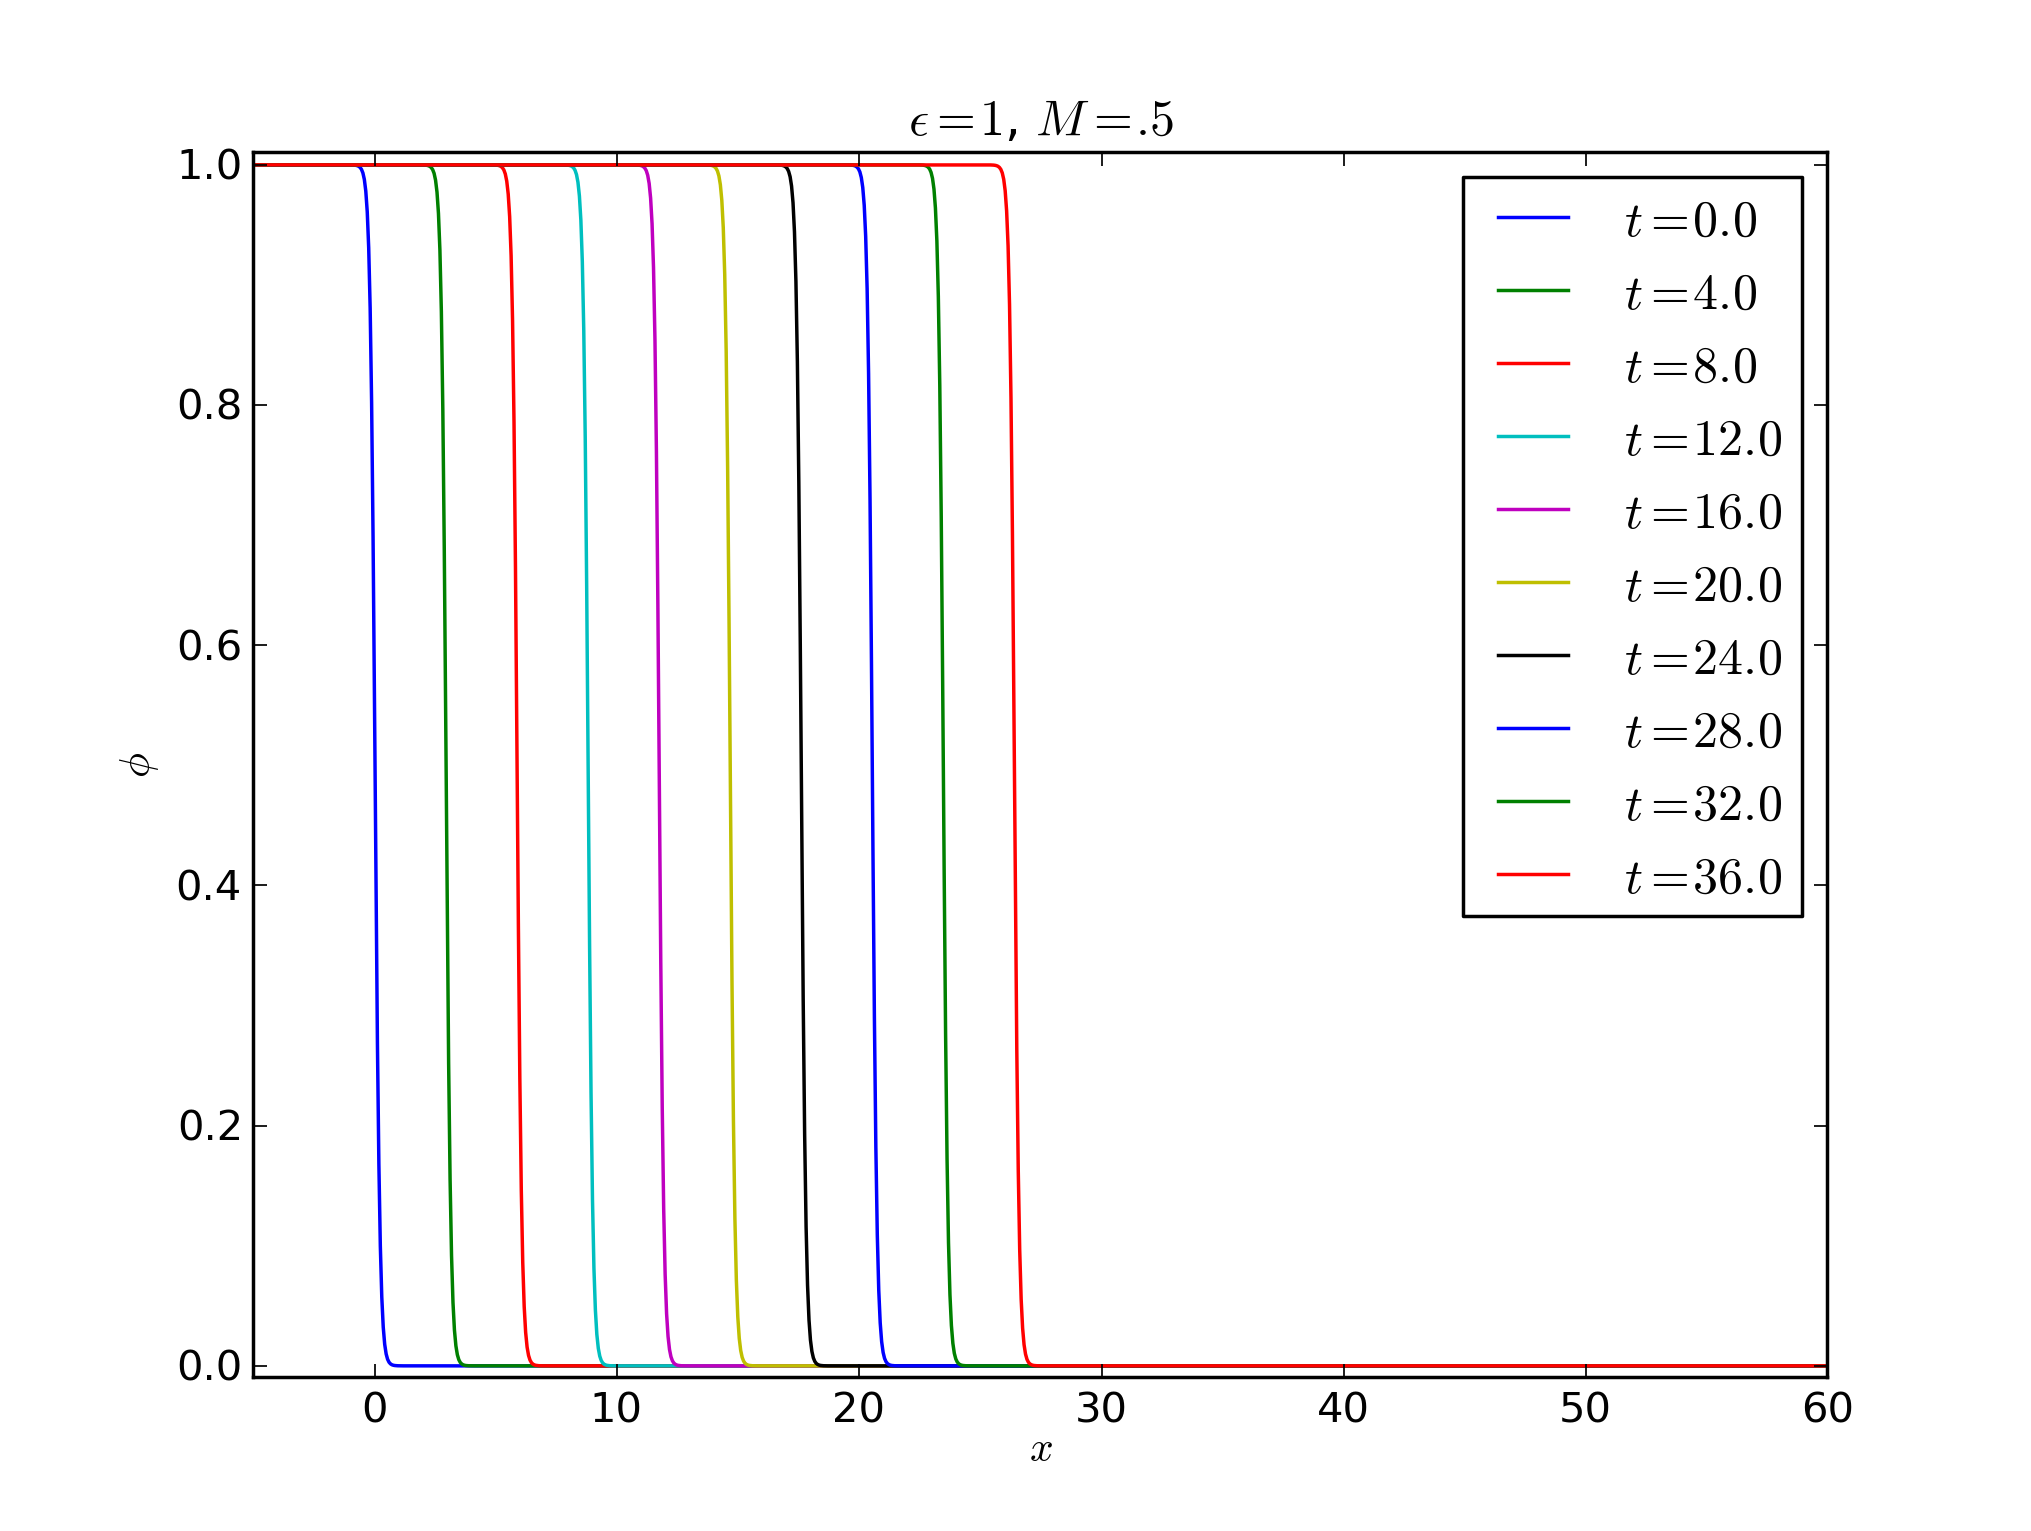
\includegraphics[width=\linewidth]{img/1D_eps1_M05}
    \caption{Evolution of $\phi$ with time for $\epsilon= 1$, $M =
    0.5$.}
    \label{fig:esp1M.5}
  \end{minipage}
\end{figure}

\begin{figure}[htbp]
  \centering
  \begin{minipage}[t]{.8\linewidth}
    \centering
    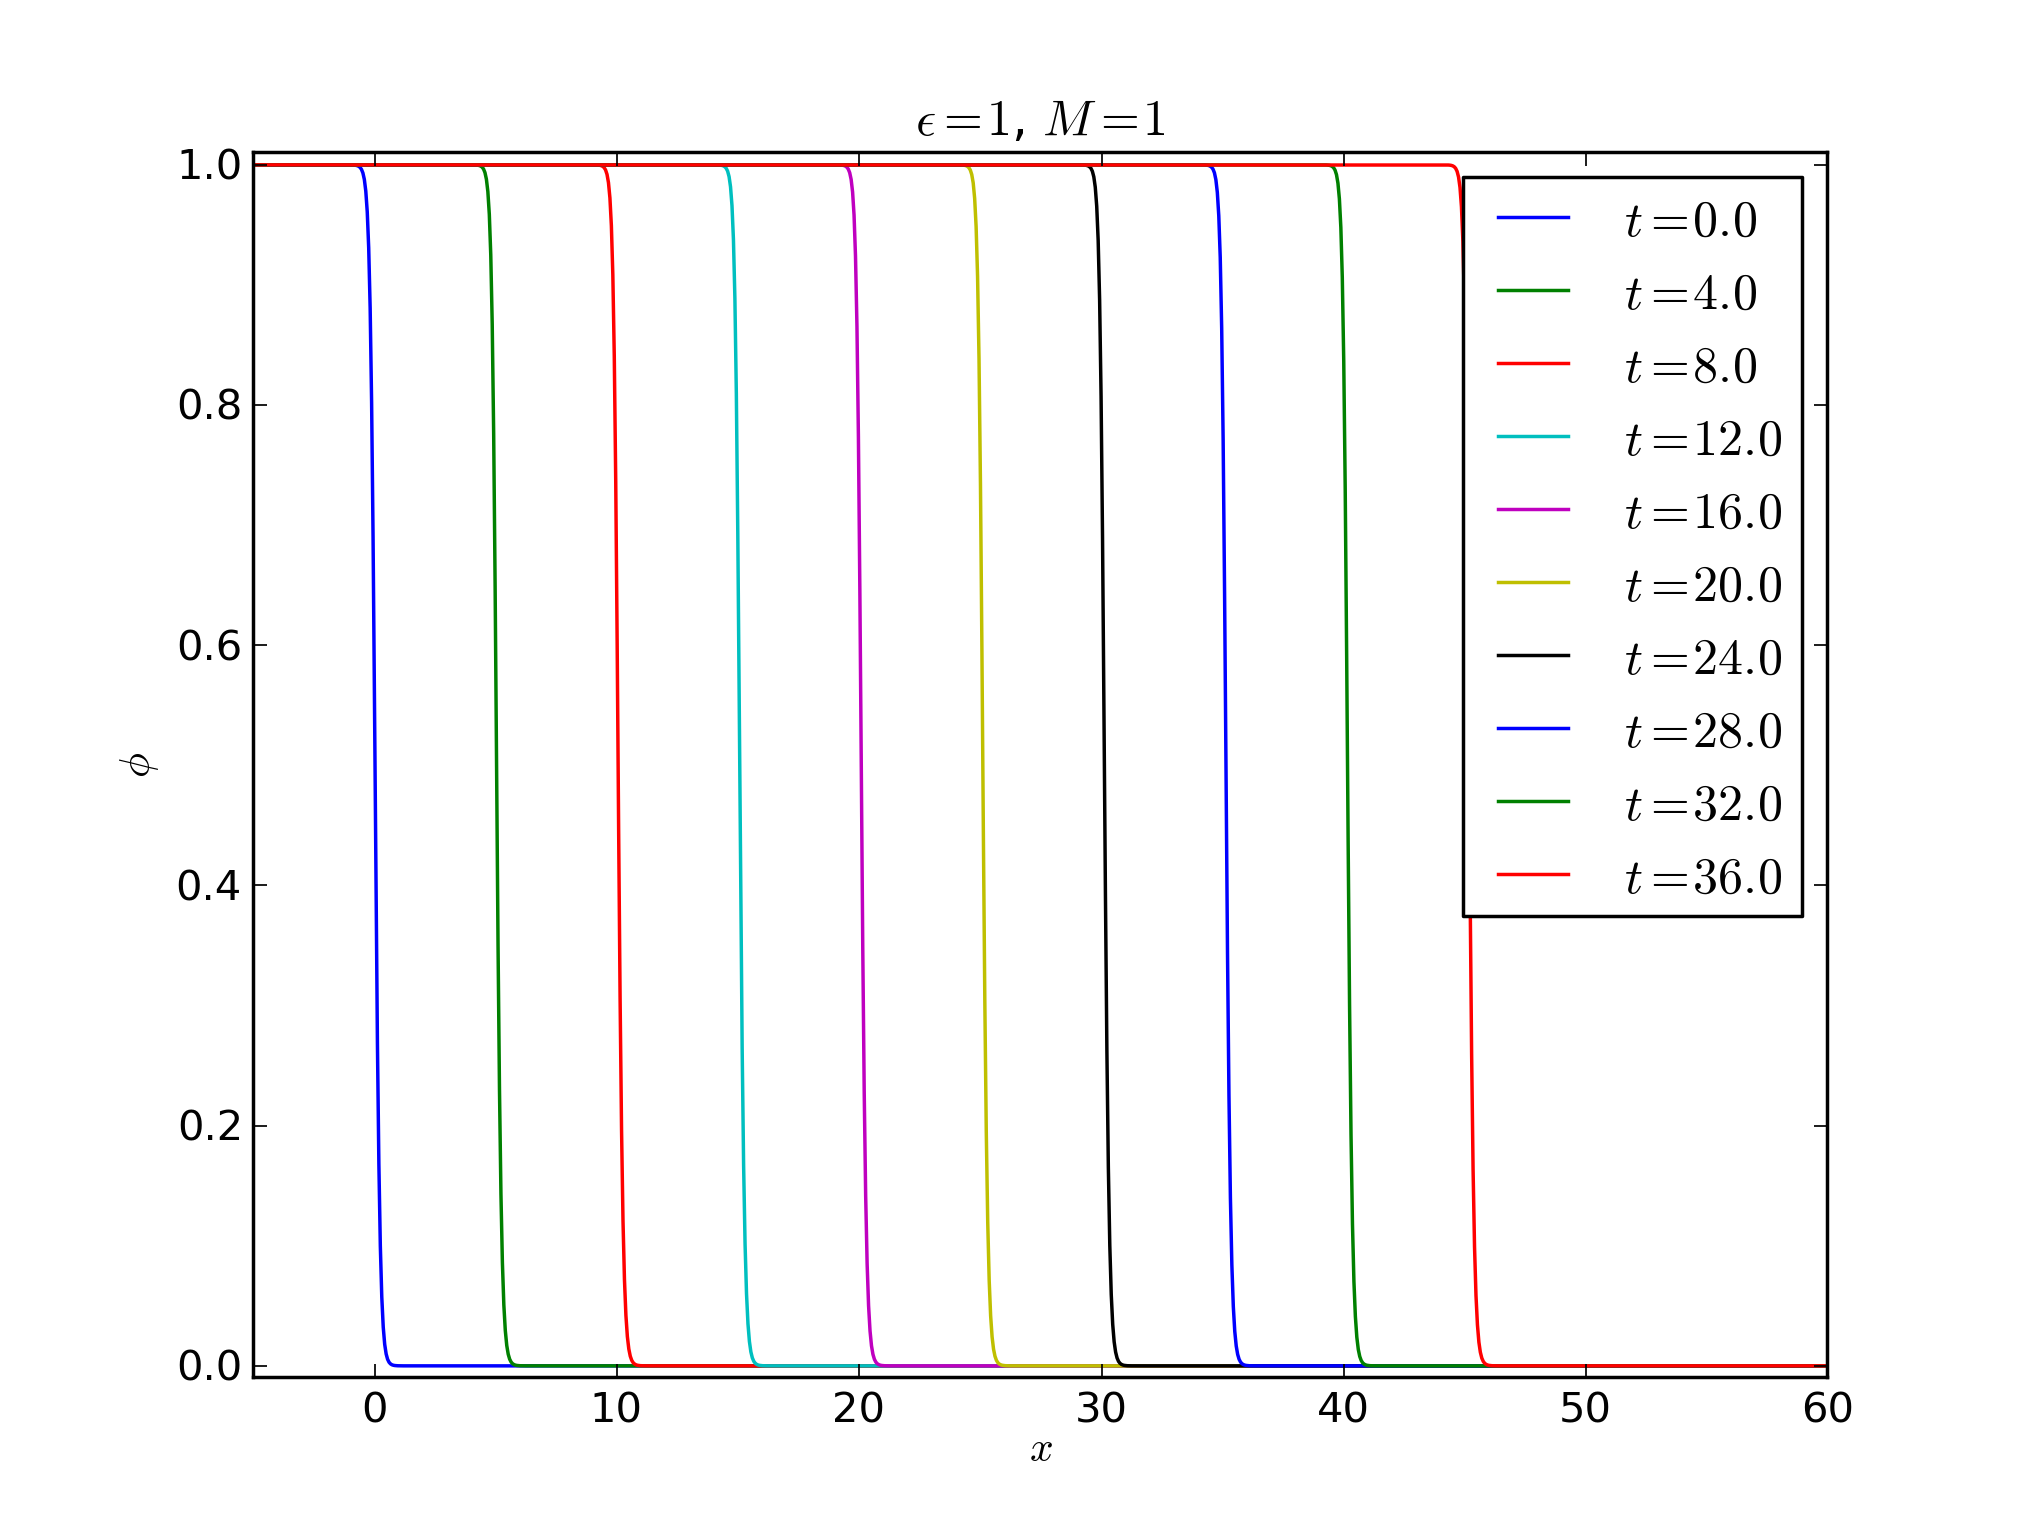
\includegraphics[width=\linewidth]{img/1D_eps1_M1}
    \caption{Evolution of $\phi$ with time for $\epsilon= 1$, $M = 1$.}
    \label{fig:esp1M1}
  \end{minipage}
\end{figure}

\begin{figure}[htbp]
  \centering
  \begin{minipage}[t]{.8\linewidth}
    \centering
    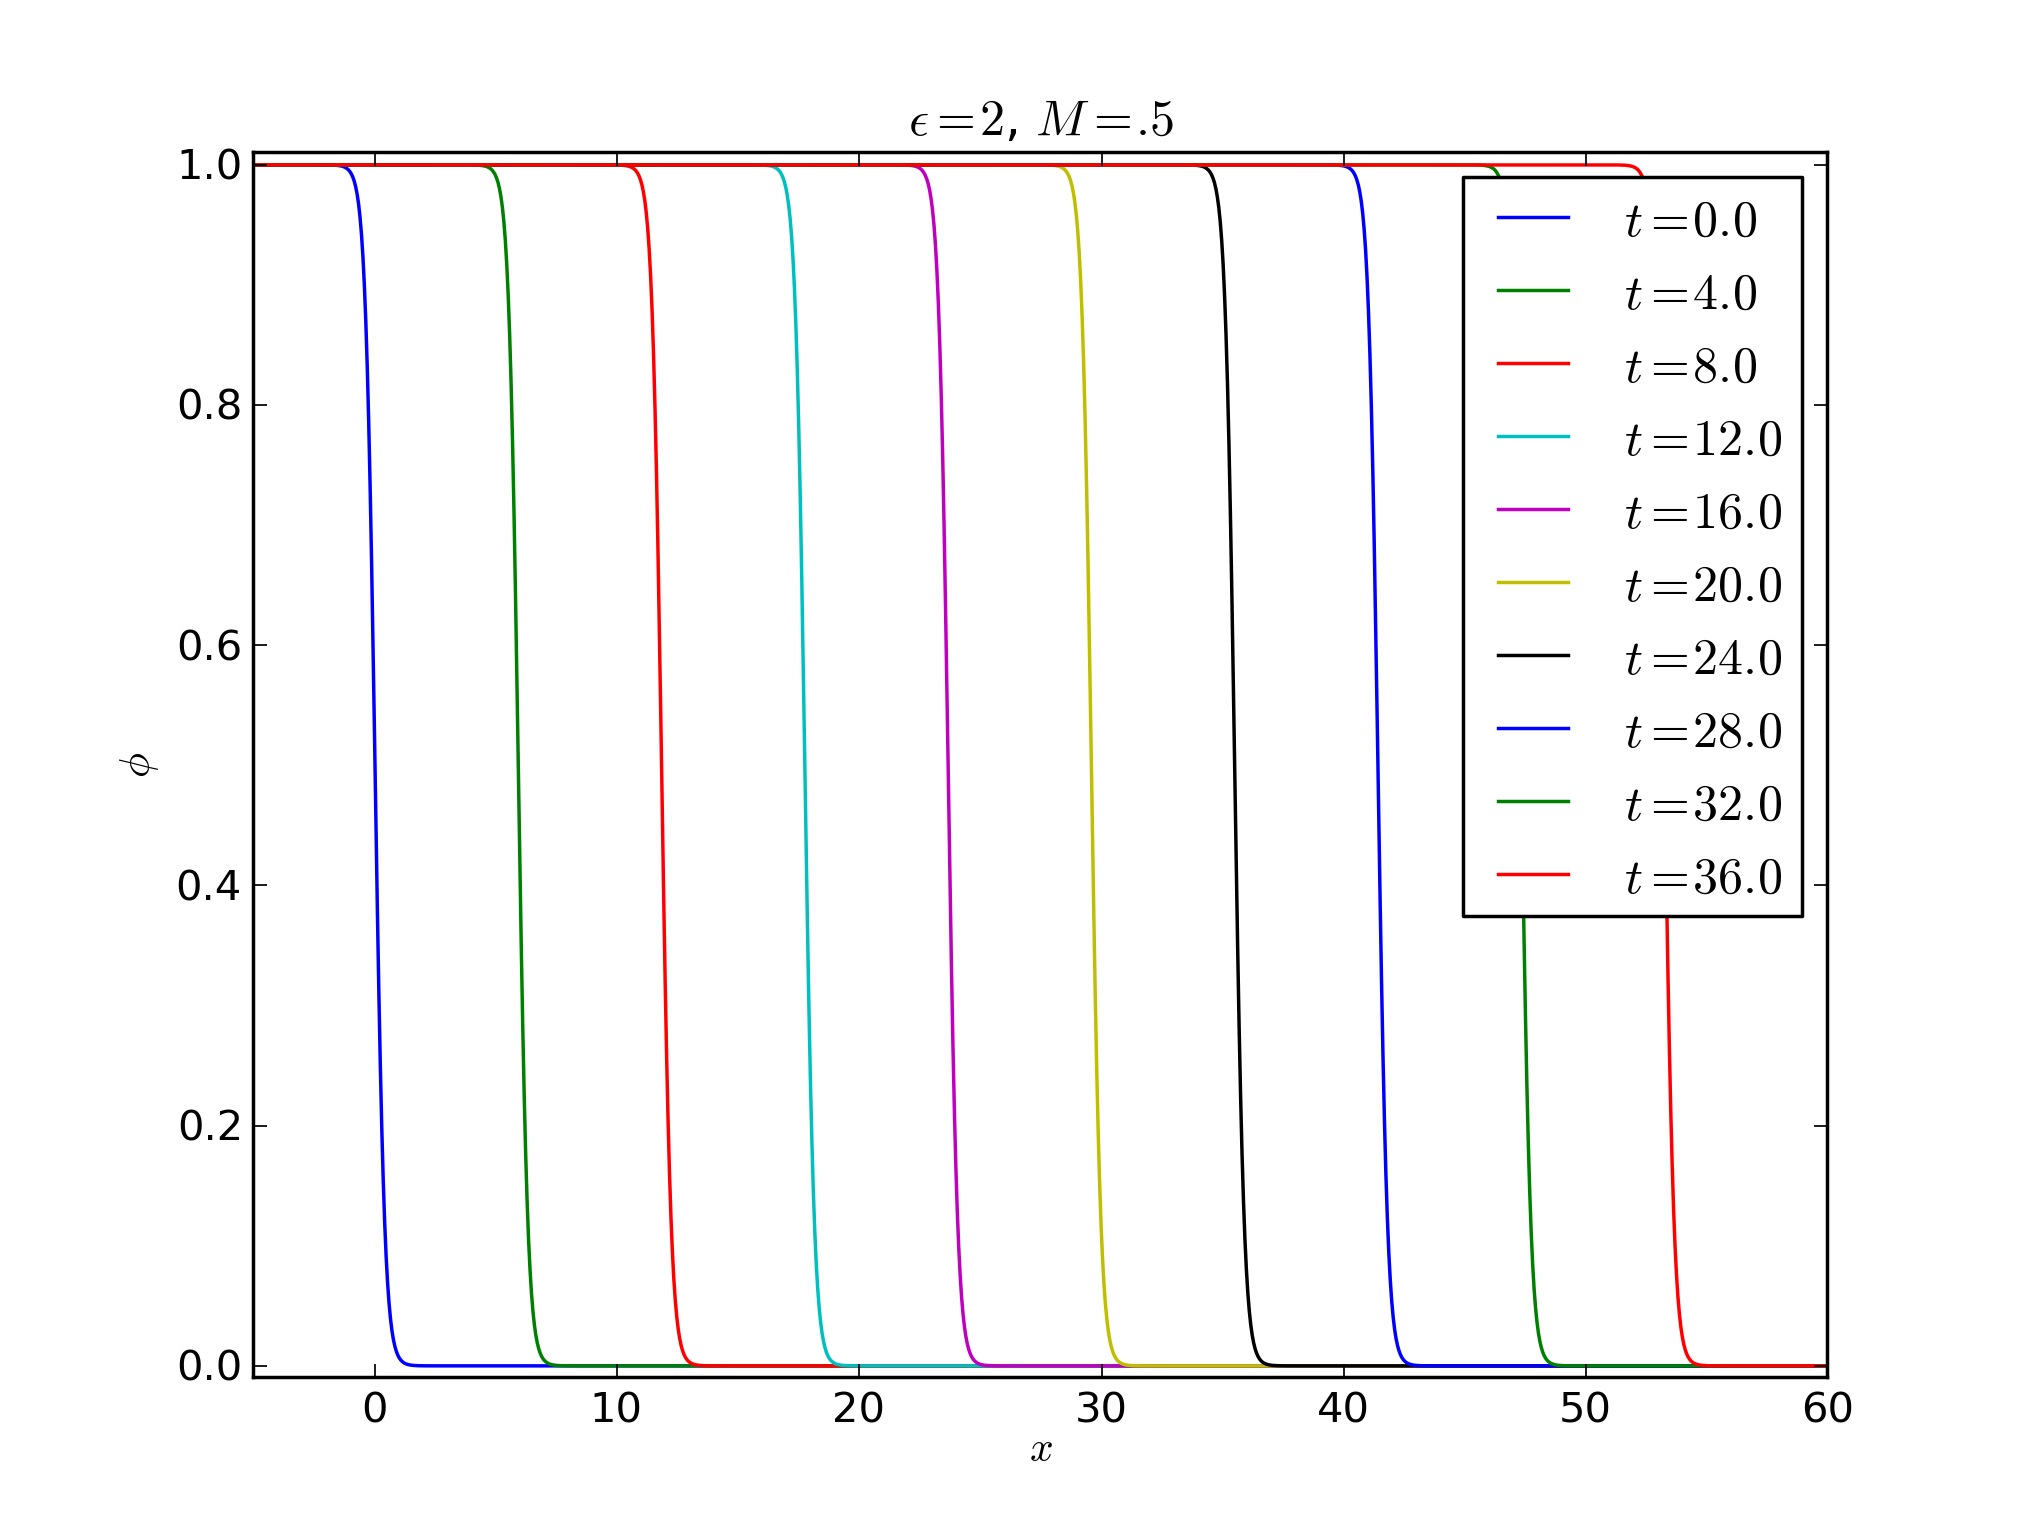
\includegraphics[width=\linewidth]{img/1D_eps2_M05}
    \caption{Evolution of $\phi$ with time for $\epsilon= 2$, $M =
    0.5$.}
    \label{fig:esp2M.5}
  \end{minipage}
\end{figure}

\bibliography{Phase_Field}
\end{document}
